%% LyX 2.4.5 created this file.  For more info, see https://www.lyx.org/.
%% Do not edit unless you really know what you are doing.
\documentclass[11pt,english]{article}
\usepackage[T1]{fontenc}
\usepackage[latin9]{inputenc}
\usepackage{babel}
\usepackage{verbatim}
\usepackage{float}
\usepackage{amsmath}
\usepackage{amssymb}
\usepackage{graphicx}
\usepackage{geometry}
\geometry{verbose,tmargin=1.1in,bmargin=1.1in,lmargin=1.1in,rmargin=1.1in}
\usepackage{setspace}
\usepackage[authoryear,round]{natbib}
\onehalfspacing
\usepackage[bookmarks=false,
 breaklinks=false,pdfborder={0 0 1},backref=section,colorlinks=false]
 {hyperref}

\makeatletter

%%%%%%%%%%%%%%%%%%%%%%%%%%%%%% LyX specific LaTeX commands.
%% Because html converters don't know tabularnewline
\providecommand{\tabularnewline}{\\}

%%%%%%%%%%%%%%%%%%%%%%%%%%%%%% User specified LaTeX commands.
\usepackage{babel}
%
\usepackage{amsfonts}
\newtheorem{prop}{Proposition}
\newtheorem{cor}{Corollary}
\newtheorem{lem}{Lemma}

\setcounter{MaxMatrixCols}{30}
\providecommand{\U}[1]{\protect\rule{.1in}{.1in}}
\newenvironment{proof}[1][Proof]{\noindent\textbf{#1.} }{\ \rule{0.5em}{0.5em}}

\newtheorem{theorem}{Theorem}
\newtheorem{acknowledgement}{Acknowledgement}
\newtheorem{algorithm}[theorem]{Algorithm}
\newtheorem{axiom}[theorem]{Axiom}
\newtheorem{assumption}{Assumption}
\newtheorem{case}[theorem]{Case}
\newtheorem{claim}[theorem]{Claim}
\newtheorem{conclusion}[theorem]{Conclusion}
\newtheorem{condition}[theorem]{Condition}
\newtheorem{conjecture}[theorem]{Conjecture}
\newtheorem{corollary}[theorem]{Corollary}
\newtheorem{criterion}[theorem]{Criterion}
\newtheorem{definition}{Definition}
\newtheorem{example}[theorem]{Example}
\newtheorem{exercise}[theorem]{Exercise}
\newtheorem{lemma}{Lemma}
\newtheorem{notation}[theorem]{Notation}
\newtheorem{problem}[theorem]{Problem}
\newtheorem{proposition}{Proposition}
\newtheorem{remark}[theorem]{Remark}
\newtheorem{solution}[theorem]{Solution}
\newtheorem{summary}[theorem]{Summary}
\usepackage{lscape}
\usepackage{placeins}
\usepackage{booktabs}
\usepackage{tabularx}
\usepackage{array}
\usepackage{microtype}
\usepackage{ragged2e}
\usepackage{tikz}
\usepackage{pgfplots}
\usepgfplotslibrary{groupplots,fillbetween}
\pgfplotsset{compat=1.18}
\newcolumntype{Y}{>{\RaggedRight\arraybackslash}X}
\setlength{\emergencystretch}{3em}
\sloppy

\makeatother

\begin{document}
\title{Necessity Entrepreneurship\thanks{We thank}}
\author{David Chivers\thanks{Department of Economics, Durham Business School, DH1 3LB, \protect\protect\href{mailto:david.chivers@durham.ac.uk}{david.chivers@durham.ac.uk}\textbf{ }}
\and Zhigang Feng\thanks{Department of Economics, University of Nebraska, Omaha, NE 68106,
United States, \protect\protect\href{mailto:z.feng2@gmail.com}{z.feng2@gmail.com}.} \and Elisa Keller\thanks{Department of Economics, University of Exeter, \protect\protect\href{mailto:elisa.keller@exeter.ac.uk}{elisa.keller@exeter.ac.uk}}
\and Bo Li\thanks{Department of Economics, Peking University, \protect\protect\href{mailto:lb.harbin@gmail.com\%5C\%2520}{lb.harbin@gmail.com }.} }
\maketitle
\begin{abstract}
This paper studies when higher entrepreneurship reflects productive
opportunity rather than weak labor-market outside options. We develop
a model of occupational choice with search frictions, unemployment
insurance, and two entrepreneurial margins: nonemployer self-employment
and employer entrepreneurship. Necessity entrepreneurs choose business
ownership only when wage-work options are weak, whereas opportunity
entrepreneurs would choose entrepreneurship even with strong outside
options. Quantitatively, lower unemployment insurance raises entrepreneurship
mainly through low-scale self-employment, while stronger labor-market
security shifts entrepreneurial activity toward employer firms and
increases aggregate output per household. The main lesson is that
the same rise in business ownership can imply very different aggregate
outcomes depending on whether it reflects improved entrepreneurial
opportunities or deteriorating labor-market insurance.

\ 

\textbf{JEL Classification}: E23, I10, O40.

\textbf{Keywords}:Occupational Choice, Entrepreneur, Misallocation, 
\end{abstract}
\pagebreak{}

\section{Introduction}

Entrepreneurship is often treated as a marker of innovation, firm
growth, and rising wages. But entrepreneurial entry can reflect very
different underlying choices: some individuals choose it despite attractive
wage-work options, while others do so only when those options are
weak or unavailable. That distinction matters for aggregate efficiency.
If business ownership rises mainly because individuals have poor outside
options, then higher entrepreneurship may reflect weak labor-market
opportunities rather than productive entrepreneurial dynamism. In
this paper, we formally distinguish between opportunity and necessity
entrepreneurship within an occupational-choice framework. Opportunity
entrepreneurs are individuals who choose entrepreneurship even when
viable wage employment is available, whereas necessity entrepreneurs
choose entrepreneurship only when it is not.

This distinction is likely to vary systematically across individuals.
The same characteristics that make an individual more productive as
an entrepreneur may also improve their prospects in wage work. If
higher human capital raises both managerial potential and labor-market
opportunities, then entrepreneurship must clear a higher bar to be
optimal. By contrast, weaker outside options may push lower-human-capital
individuals into entrepreneurial activity under less favorable conditions.
As a result, changes in entrepreneurial entry can have very different
aggregate implications depending on who enters and what type of business
activity they undertake.

The difficulty is that this distinction is not directly observed.
Empirical work has therefore relied on indirect measures, but these
do not cleanly uncover the underlying occupational-choice object.
One approach uses stated motives. In weighted U.S. GEM APS microdata
for 2019--2021, between 41 and 50 percent of early-stage entrepreneurs
report starting a business because jobs are scarce, while between
65 and 73 percent also report motives tied to building wealth or very
high income. These responses are informative, but they do not deliver
a clean classification: necessity and opportunity signals can coexist
within the same entrepreneurial spell. A second approach classifies
entrepreneurs by prior labor-market status. That is also useful, but
observed status at entry is not the object we seek to identify. Workers
may start a business while still employed because they anticipate
worsening job prospects, while some more growth-oriented entrepreneurs
may pass through temporary non-employment before starting a firm.

What is missing, however, is a definition of this distinction at the
level of occupational choice. In the model below, entrepreneurship
can take the form of nonemployer self-employment or employer entrepreneurship.
This allows the framework to speak not only to entrepreneurial entry,
but also to the composition and scale of entrepreneurial activity.
In particular, it can distinguish between an increase in low-scale
business ownership driven by weak outside options and an increase
in employer-oriented entrepreneurship driven by stronger entrepreneurial
prospects.

The paper makes three contributions. First, it offers a formal definition
of necessity entrepreneurship grounded in optimal occupational choice
rather than stated motives or prior labor-market status. Second, it
develops a theoretical framework that embeds search and matching frictions
within a span-of-control model of occupational choice, so the wage-work
outside option is endogenous to labor-market conditions. Third, the
quantitative results show that policy-induced increases in entrepreneurship
operate mainly through a compositional margin: weaker outside options
raise low-scale self-employment much more than employer entrepreneurship.
This is why the paper emphasizes entrepreneurial composition, scale,
and aggregate output rather than the entrepreneurship rate alone.

The remainder of the paper is organized as follows. Section 2 presents
the empirical motivation. Section 3 discusses the related literature.
Section 4 sets out the model environment. Section 5 characterizes
equilibrium. Section 6 discusses calibration. Section 7 presents the
quantitative results. Section 8 studies policy counterfactuals. Section
9 concludes.

\section{Empirical Motivation}

Necessity entrepreneurship is difficult to identify cleanly in observed
data. But recessions are informative because they weaken outside options
in wage employment.

Figure 1 shows this pattern in business stocks. During the Great Recession,
zero-employee establishments rose by 1.85 percent, while businesses
with employees contracted. The decline was largest among establishments
with 20 or more employees, which fell by 5.82 percent. Lower-scale
business ownership was therefore comparatively resilient even as employer
firms weakened. This does not mean that nonemployer businesses directly
measure necessity entrepreneurship. It does suggest that downturns
shift entrepreneurial activity toward smaller-scale ownership rather
than employer growth.

\begin{figure}[H]
\begin{centering}
\caption{U.S. business counts by employment size, indexed to 1997.}
\par\end{centering}
\centering{}% Auto-generated by pull_us_business_size_cycle_data.py
\begin{tikzpicture}
\begin{axis}[
width=0.82\textwidth,
height=0.50\textwidth,
title={US business counts by employment size},
ylabel={Index (1997=100)},
xlabel={},
xmin=1997, xmax=2022,
ymin=94.4149, ymax=198.6696,
xtick={1997,2002,2007,2012,2017,2022},
xticklabel style={/pgf/number format/fixed},
ymajorgrids=true,
grid style={gray!30},
tick align=outside,
axis line style={black!70},
tick style={black!70},
legend cell align={left},
legend style={draw=none, fill=none, at={(0.02,0.98)}, anchor=north west, font=\small},
]
\path[fill=gray!18,draw=none] (axis cs:2000.5,94.4149) rectangle (axis cs:2001.5,198.6696);
\path[fill=gray!18,draw=none] (axis cs:2007.5,94.4149) rectangle (axis cs:2008.5,198.6696);
\path[fill=gray!18,draw=none] (axis cs:2008.5,94.4149) rectangle (axis cs:2009.5,198.6696);
\path[fill=gray!18,draw=none] (axis cs:2019.5,94.4149) rectangle (axis cs:2020.5,198.6696);
\addplot[very thick, color=blue!65!black] table [x=year, y=establishments_0_index_1997, col sep=comma] {../data/us_business_counts_by_size_annual.csv};
\addplot[very thick, color=green!45!black] table [x=year, y=establishments_1_4_index_1997, col sep=comma] {../data/us_business_counts_by_size_annual.csv};
\addplot[very thick, color=orange!85!black] table [x=year, y=establishments_5_19_index_1997, col sep=comma] {../data/us_business_counts_by_size_annual.csv};
\addplot[very thick, color=red!65!black] table [x=year, y=establishments_20_plus_index_1997, col sep=comma] {../data/us_business_counts_by_size_annual.csv};
\legend{0 employees,1--4 employees,5--19 employees,20+ employees}
\end{axis}
\end{tikzpicture}

\end{figure}

Figure 2 shows the same pattern in business formation flows. Total
business applications fell by 5.84 percent during the recession, but
high-propensity applications fell by 22.12 percent, and their share
of total applications also declined sharply. The recession therefore
did not simply reduce entry in the aggregate; it shifted new business
formation away from the employer-oriented margin.

\begin{figure}[H]
\begin{centering}
\caption{U.S. business applications and the high-propensity share.}
\par\end{centering}
\centering{}% Auto-generated by pull_us_business_applications_companion.py
\begin{tikzpicture}
\begin{groupplot}[
group style={group size=1 by 2, vertical sep=0.95cm},
width=0.82\textwidth,
height=0.28\textwidth,
xmin=2005, xmax=2025,
xtick={2005,2010,2015,2020,2025},
xticklabel style={/pgf/number format/fixed},
ymajorgrids=true,
grid style={gray!30},
tick align=outside,
axis line style={black!70},
tick style={black!70},
]
\nextgroupplot[
ylabel={Index (2005=100)},
xlabel={},
ymin=69.5481, ymax=234.1728,
xticklabel=\empty,
legend cell align={left},
legend style={draw=none, fill=none, at={(0.02,0.98)}, anchor=north west, font=\small},
]
\path[fill=gray!18,draw=none] (axis cs:2007.5,69.5481) rectangle (axis cs:2008.5,234.1728);
\path[fill=gray!18,draw=none] (axis cs:2008.5,69.5481) rectangle (axis cs:2009.5,234.1728);
\path[fill=gray!18,draw=none] (axis cs:2019.5,69.5481) rectangle (axis cs:2020.5,234.1728);
\addplot[very thick, color=black!75] table [x=year, y=applications_total_index_2005, col sep=comma] {../data/us_business_applications_annual.csv};
\addplot[very thick, color=orange!85!black] table [x=year, y=applications_high_propensity_index_2005, col sep=comma] {../data/us_business_applications_annual.csv};
\legend{Total applications,High-propensity applications}
\nextgroupplot[
ylabel={Share (\%)},
xlabel={},
ymin=28.1807, ymax=61.0054,
]
\path[fill=gray!18,draw=none] (axis cs:2007.5,28.1807) rectangle (axis cs:2008.5,61.0054);
\path[fill=gray!18,draw=none] (axis cs:2008.5,28.1807) rectangle (axis cs:2009.5,61.0054);
\path[fill=gray!18,draw=none] (axis cs:2019.5,28.1807) rectangle (axis cs:2020.5,61.0054);
\addplot[very thick, color=teal!60!black, mark=*, mark size=1.7pt] table [x=year, y expr=\thisrow{high_propensity_share}*100, col sep=comma] {../data/us_business_applications_annual.csv};
\end{groupplot}
\end{tikzpicture}

\end{figure}

Taken together, the figures motivate the paper\textquoteright s main
measurement point: different empirical measures capture different
margins of entrepreneurship, and these should not be treated as economically
equivalent. The framework developed below is designed to explain these
compositional differences rather than a single aggregate entrepreneurship
statistic.

\section{Literature Review}

This paper relates most directly to the literature distinguishing
opportunity from necessity entrepreneurship. Much of the empirical
literature operationalizes this distinction using observable proxies,
especially stated motives or pre-entry labor-market status. \citet{fairlie_fossen_2019}
propose an objective classification based on pre-entry work status
and show that opportunity and necessity entry display different cyclical
patterns. \citet{fairlie_2013} and \citet{fossen_2021} likewise show
that entrepreneurial entry is heterogeneous over the cycle, with unemployment-driven
and lower-scale entry behaving differently from more growth-oriented
business creation. Using GEM microdata, \citet{chivers_2017} show
that necessity entrepreneurship is negatively associated with economic
development, whereas opportunity entrepreneurship is positively associated
with development. \citet{poschke_2013} provide the closest bridge
from these empirical patterns to a structural interpretation by emphasizing
how labor-market prospects shape entrepreneurial selection, and \citet{levine_rubinstein_2020}
further show that entrepreneurship and other forms of self-employment
should not be treated as interchangeable objects. This literature
makes clear that entrepreneurial entry is heterogeneous, but it usually
measures that heterogeneity through reduced-form proxies rather than
through the occupational-choice problem itself.

The paper also builds on the occupational-choice tradition in macroeconomics
and entrepreneurship. \citet{lucas_1978}, \citet{evans_jovanovic_1989},
and \citet{buera_2009} show why entrepreneurial selection, firm scale,
and financial constraints should be studied jointly rather than through
entry alone. \citet{hurst_pugsley_2011} add an important empirical
qualification: much small-business activity is not well described
by the standard high-growth view of entrepreneurship. That point is
central here. If weaker outside options raise primarily low-scale
self-employment rather than employer entrepreneurship, then the relevant
outcome is not simply whether business ownership rises, but which
type of business activity expands and with what implications for firm
scale, output, and welfare.

The paper also relates to a smaller but growing literature that embeds
self-employment in equilibrium search environments. \citet{mortensen_pissarides_1994}
and \citet{petrongolo_pissarides_2001} provide the benchmark search-and-matching
framework for job-finding rates, separations, and labor-market tightness.
\citet{albrecht_navarro_vroman_2009} and \citet{satchi_temple_2009}
show that in economies with formal and informal sectors, search frictions
shape the allocation of workers across unemployment, wage work, and
self-employment. \citet{narita_2020}, \citet{denderski_sniekers_2024},
and \citet{poschke_2025} move closer to the present paper by modeling
self-employment as an alternative to job search and showing that changes
in labor-market frictions materially affect self-employment outcomes.
\citet{chodorow_reich_karabarbounis_2016} add that the opportunity
cost of employment is itself cyclical, while \citet{hombert_schoar_sraer_thesmar_2020}
show that unemployment insurance can raise entrepreneurial entry by
reducing downside risk. The present paper brings these strands together
in a setting where job-finding risk, separation risk, and unemployment
insurance jointly shift the occupational-choice threshold, making
the distinction between opportunity and necessity entrepreneurship
endogenous to labor-market conditions.

The paper also relates to the literature on entrepreneurial composition
over the business cycle. \citet{sedlacek_sterk_2017} show that startup
employment is procyclical and that cohort differences reflect startup
size and growth potential, not only startup counts. \citet{haltiwanger_jarmin_miranda_2013}
and \citet{fort_etal_2013} similarly show that young firms, startup
job creation, and firm scale respond strongly to cyclical conditions.
This evidence suggests that changes in entrepreneurship should not
be interpreted through a single extensive-margin statistic. That perspective
aligns closely with the central prediction of this paper: weaker outside
options can increase lower-scale business ownership even when employer-oriented
entry or startup growth potential weakens.

Relative to these literatures, the paper contributes in two ways. First,
it offers a structural definition of necessity entrepreneurship grounded
in optimal occupational choice rather than in motives or prior status
alone. Second, it embeds that distinction in a framework with heterogeneous
human capital, entrepreneurial ability, search frictions, closure
risk, and social insurance, allowing the model to speak not only
to entrepreneurial entry, but also to entrepreneurial composition,
firm scale, and the distinction between self-employment and employer
entrepreneurship.

\section{The Model: Economic Environment}

Consider a Lucas (1978) span of control model, where individuals differ
in the level of human capital, $h.$ As in Gomez and Kuhen (2017),
individuals are educated to either the primary $(P)$, secondary $(S)$
or tertiary level $(T)$. The level of education means that a tertiary
educated individuals have a higher draw of human capital, on average,
than secondary educated individuals, who in turn have a higher draw
on average than primary educated individuals. This human capital draw
is positively correlated with managerial ability $x$ as well as labor
productivity $z$.

At the start of the period agents enter as either unemployed $($$i_{w}=0)$,
employed $($$i_{w}=1)$, or an entrepreneur $($$i_{w}=2)$. Individuals
face a choice of whether to become an entrepreneur, to continue working
or to search for work. However, the value of employment is different
depending on whether an agent enters the period as employed $($$i_{w}=1)$
or not. Although there is a risk that an employee may become separated
from a firm with probability $\rho$, this is less risky than searching
for work which has a $p(\theta)$ probability of obtaining employment.
Consequently, the expected value of employment is higher for those
already in employment than those who are not. Additionally, the probability
of separation is lower for individuals with higher levels of human
capital and they are able to command a higher wage due to higher levels
of productivity. So the value of employment, holding other things
equal, is higher for those with higher human capital as well.

The innovation of this model is that the entrepreneurial decision
results in two types of entrepreneurs emerge, opportunity-based entrepreneurs
and necessity-based entrepreneurs. We define opportunity-based entrepreneurs
are those whose value of entrepreneurship is higher, even if they
had employment. Necessity-based entrepreneurs are those who would
not have become entrepreneurs, if they had employment.

\paragraph{Timing: }

The timing of events can be summarized below. Occupational choice
happens at the start of time $t.$ Those choosing to become entrepreneurs
run projects and choose capital and hired labor each period. If hired
labor satisfies $n_{h}=0$ the business is nonemployer self-employment,
while $n_{h}>0$ corresponds to employer entrepreneurship. Entrepreneurial
businesses face closure risk $\rho_{e}(h)$ . In the benchmark, closure
moves the household out of business and into non-employment without
automatic regular unemployment insurance eligibility. Those who were
previously employed within a project can decide to carry on working
but carry a risk of separation with probability $\rho$. If separation
occurs these workers will claim unemployed benefits and be unable
to look for work until the following period. After separation occurs,
vacancies are posted and who were unemployed in the previous period
are matched with firms. Those that are successful and match with with
probability $p(\theta)$ go on to earn a wage. Whereas those that
are unsuccessful will claim unemployment benefits and be unable to
search again until the following period.~

Unlike the search and matching literature there is no wage bargaining
between workers and the firm at the end of matching. Instead the wage
pins down the occupational choice decision which determines those
wanting to become entrepreneurs and those who will search for work.
Crucially, the worker only finds out whether they enter production
and earn a wage after their occupational choice decision.

\begin{figure}[H]
\begin{centering}
\caption{Timing for Matched Workers}
\par\end{centering}
\centering{}
\includegraphics[width=0.82\textwidth]{../figures/enter_period_employed_submission} 
\end{figure}

\begin{figure}[H]
\begin{centering}
\caption{Timing for Unmatched Workers}
\par\end{centering}
\centering{}
\includegraphics[width=0.82\textwidth]{../figures/enter_period_unemployed_submission} 
\end{figure}


\subsection{Preferences, endowments and technology}

\paragraph{Preferences: }

Consumption by an agent in period $t$ is $c_{t}$, with utility given
by $U(c_{t})$.

\paragraph{Endowments: }

Agents are endowed with an initial capital asset, $a_{0}$, which
can be used as an input in production. Each individual is endowed
with human capital shock $h^{i}$. Human capital $h$ is positively
correlated with managerial talent $x$, labor productivity $z$ and
separation rate $\rho.$

\paragraph{Production: }

Firms use labor $n$ and capital $k$ to produce a single consumption
good, $y$. Capital depreciates at a constant rate of $\delta$.Managers
can operate only one project.The functional form of the production
function is: 
\begin{equation}
y=xk^{\alpha}\left(\ell_{e}+\xi zn_{h}\right)^{\gamma}\ \ \mbox{where}\ \alpha,\gamma>0.\ \label{eq:firm_prod}
\end{equation}
 so self-employment is feasible at $n_{h}=0$ , while employer entrepreneurship
corresponds to $n_{h}>0$ . Managerial talent $x$ is determined by
the Pareto distribution $F(x)=\left[1+\frac{x-\varsigma}{\xi}\right]^{-\vartheta_{i}}$
where $\vartheta$ is the shape parameter, $\varsigma$ the location
parameter and $\xi$ is the scale parameter.

\paragraph{Factor remuneration: }

Firms rent capital at the common market rate $r$.

\paragraph{Government:}

The government runs a balanced budget each period and provides unemployment
insurance which is financed through lump sum taxation $\tau$, which
is shared by the employee $(1-\psi)\tau$ and employer $\psi\tau$.
This program guarantees each household an unemployment benefit of
$b$.

\subsection{The Firm's problem}

The firm's problem is: 
\begin{equation}
\max_{n,k}Xk^{\alpha}n^{\gamma}-(1+\tau\psi)wzn-rk-\kappa\frac{\rho zn}{q(\theta_{t})}\label{eq:max_firm}
\end{equation}
employees must pay a share of unemployment insurance $\tau$ to all
workers who produce output. Firms have to pay search costs $\kappa$
for all vacancies posted. The number of vacancies posted is designed
to replace any lost workers, $\rho zn.$ This, however, is affected
by the firm-hiring rate $q(\theta_{t})=\bar{m}\left(\frac{v_{t}}{u_{t}}\right)^{-\mu}$,
where aggregate vacancies $v_{t}$ is simply the aggregate level of
all those who have separate from firms $\sum\rho zn$ within the period
and $u_{t}$ is the total unemployed looking for work within that
period (see appendix).

When the market is tight and the hiring rate is low, firms have to
search more and thus face higher search costs in order to replace
lost workers. $\text{This is because }0<q(\theta_{t})<1,$so a lower
$q(\theta_{t})$ increases $\frac{\rho zn}{q(\theta_{t})}$. If the
firm lose 10 workers, they want to hire 10 workers to replace them.
But if the hiring rate, $q(\theta_{t}),$ is 50\% then they will face
double the amount of search costs than if $q(\theta_{t})$ were 100\%.
The upshot of this is that when markets are tight, the size of the
desired firm size $n$ decreases ex ante , as the cost of replacing
workers is high and so entrepreneurs would prefer to run smaller firms.

To avoid issues of directed search, we assume that employees are randomly
matched with firms (as in Chivers et al., 2015) and each firm employees
a distribution of workers across the human capital spectrum such that
each firm employs the market average.

\section{Optimal behavior and equilibrium}

In any time period $t$ agents are distinguished by $(h,a,x,i,z)$.
The timing of the economy is given as follows. 
\begin{enumerate}
\item Households enter each new period with assets $a$ and an employment
status $i_{w}$ 
\item Idiosyncratic shocks $h$ is drawn which determines $x$ (managerial
ability) and $z$ (labor productivity), $\rho$ seperation rate conditional
on education level, $P,S$ or $T.$ 
\item Households make an occupation decision: entrepreneur ($\mathcal{I}_{e}=1$)
or worker ($\mathcal{I}_{e}=0$). 
\item Capital and labor markets clear. A fraction $\rho$ of employees separate
from firms and~$p(\theta)$ are hired to replace them 
\item Households choose: consumption ($c$), borrowing/saving ($a'$) 
\end{enumerate}

\subsection{Firm manager}

Firms are distinguished by their productivity realization $x$. In
the self-employment version, entrepreneurs choose capital and hired
labor while also supplying owner labor to the business. Let $n_{h}$
denote hired labor and $\ell_{e}$ denote owner labor. When $n_{h}=0$
the entrepreneur is self-employed; when $n_{h}>0$ the entrepreneur
is an employer. The static problem for a manager with talent $x^{i}$
is  
\begin{equation}
\max_{k,n_{h}\geq0}xk^{\alpha}\left(\ell_{e}+\xi zn_{h}\right)^{\gamma}-zw(1+\psi\tau)n_{h}-rk-\kappa\frac{\rho zn_{h}}{q(\theta)}-f_{hire}\mathbf{1}\{n_{h}>0\}\label{maxP}
\end{equation}

Self-employment is therefore the corner $n_{h}=0$ , while employer
entrepreneurship corresponds to $n_{h}>0$ . For an interior employer
choice, the first-order condition for hired labor is:

\begin{equation}
\gamma xk^{\alpha}\left(\ell_{e}+\xi zn_{h}\right)^{\gamma-1}\xi z=w(1+\psi\tau)+\frac{\rho\kappa}{q(\theta)}\label{maxP-1}
\end{equation}

\begin{equation}
n^{*}_{h}(k,x,\widetilde{w})=\max\left\{ 0,\frac{1}{\xi z}\left[\left(\frac{\gamma xk^{\alpha}\xi z}{w(1+\psi\tau)+\frac{\rho\kappa}{q(\theta)}}\right)^{\frac{1}{1-\gamma}}-\ell_{e}\right]\right\} \label{FOC}
\end{equation}

Substituting (\ref{FOC}) into (\ref{maxP}) yields the entrepreneur's
profit function: 
\begin{equation}
\pi(k,n^{*}_{h},x;\widetilde{w})=xk^{\alpha}\left(\ell_{e}+\xi zn^{*}_{h}\right)^{\gamma}-zn^{*}_{h}w(1+\psi\tau)-rk-\kappa\frac{\rho zn^{*}_{h}}{q(\theta)}-f_{hire}\mathbf{1}\{n^{*}_{h}>0\}\label{profitj}
\end{equation}


\subsubsection{Capital}

Initially we assume capital markets function perfectly, so the interior
capital choice satisfies
\[
\alpha xk^{\alpha-1}\left(\ell_{e}+\xi zn_{h}\right)^{\gamma}=r.
\]


\subsection{Entrepreneurs}

Entrepreneurs maximize expected discounted utility of consumption
\[
\text{with }n_{h}=0\text{ denoting nonemployer self-employment and }n_{h}>0\text{ denoting employer entrepreneurship.}
\]
\[
\max_{\{c_{t},a_{t+1},k_{t},n_{h,t}\}}\mathbb{E}\sum^{\infty}_{t=0}\beta^{t}U(c_{t})
\]
subject to the following budget constraint: 
\begin{align}
c+a' & \leq(1+r-\delta)a+\pi(k,n_{h},x;\tilde{r},w,\tau)-\tau_{\pi}\label{eq:c_worker-3}
\end{align}

\[
a'\geq-\bar{a}
\]


\subsection{Employed}

The workforce (previous periods employed who choose to reapply for
work) maximize expected discounted utility of consumption 
\[
\max_{\{c_{t},a_{t+1}\}}\mathbb{E}\sum^{\infty}_{t=0}\beta^{t}U(c_{t})
\]
subject to the following budget constraint: 
\begin{align}
c+a' & \leq(1+r-\delta)a+(1-\rho)\left(wz(1-(1-\psi)\tau_{y})\right)+\rho b\label{eq:c_worker}
\end{align}

\[
a'\geq-\bar{a}
\]
where $b$ is the unemployment benefit.

\subsection{Unemployed}

The unemployed maximize expected discounted utility of consumption
\[
\max_{\{c_{t},a_{t+1}\}}\mathbb{E}\sum^{\infty}_{t=0}\beta^{t}U(c_{t})
\]
subject to the following budget constraint: 
\begin{align}
c+a' & \leq(1+r-\delta)a+p(\theta)\left(wz(1-(1-\psi)\tau_{y})\right)+(1-p(\theta))b\label{eq:c_worker-2}
\end{align}

\[
a'\geq-\bar{a}
\]
where $b$ is the unemployment benefit.

\subsection{Government }

The government runs a balanced budget with a lump-sum taxes $T(y)=(y-\lambda_{p}y^{1-\tau_{p}})$

\subsection{The household's problem}

Let $i_{w}$ denote the household's labor market status in the previous
period, with $i_{w}=2$ indicating being entrepreneur, $i_{w}=1$
being employed and $i_{w}=0$ being unemployed. Let $\mathcal{I}_{e}$
indicate occupational choice, where $\mathcal{I}_{e}=1$ if the household
is an entrepreneur and $\mathcal{I}_{e}=0$ if the household is a
worker.

Let $\mathbb{E}_{\rho(h)}$ denote the continuation operator for employed
workers who face job separation, let $\mathbb{E}_{p(\theta)}$ denote
the continuation operator for households searching for work, and let
$\mathbb{E}_{\rho_{e}(h)}$ denote the continuation operator for entrepreneurs
facing business closure. We write $\mathbf{V}_{0}$ for the continuation
value after business closure; in the benchmark this state does not
automatically receive regular unemployment insurance. More specifically,
\begin{align*}
\mathbb{E}_{p(\theta)}\mathbf{V}(a',h,x',i'_{w}) & =p(\theta)\mathbf{V}(a',h,x',i'_{w}=1)+(1-p(\theta))\mathbf{V}(a',h,x',i'_{w}=0)
\end{align*}

\begin{align*}
\mathbb{E}_{\rho(h)}\mathbf{V}(a',h,x',i'_{w}) & =(1-\rho(h))\mathbf{V}(a',h,x',i'_{w}=1)+\rho(h)\mathbf{V}(a',h,x',i'_{w}=0)
\end{align*}

\begin{align*}
\mathbb{E}_{\rho_{e}(h)}\mathbf{V}(a',h,x',i'_{w}) & =(1-\rho_{e}(h))\mathbf{V}(a',h,x',i'_{w}=2)+\rho_{e}(h)\mathbf{V}_{0}(a',h,x',i'_{w}=0)
\end{align*}

\begin{align*}
\mathbf{V}(a,h,x,i_{w}) & =\max\left\{ V^{w}(a,h,x,i_{w}),V^{e}(a,h,x)\right\} \\
V^{w}(a,h,x,i_{w}) & =\max_{\left\{ a',c\right\} }\left\{ u(c)+\iota_{i_{w}=1}\beta\mathbb{E}_{\rho(h)}\mathbf{V}(a',h,x',i'_{w})+\iota_{i_{w}\neq1}\beta\mathbb{E}_{p(\theta)}\mathbf{V}(a',h,x',i'_{w})\right\} \\
V^{e}(a,h,x) & =\max_{\left\{ a',c,k,n_{h}\geq0\right\} }\left\{ u(c)+\chi_{se}\mathbf{1}\{n_{h}=0\}+\chi_{emp}\mathbf{1}\{n_{h}>0\}+\beta\mathbb{E}_{\rho_{e}(h)}\mathbf{V}(a',h,x',i'_{w})\right\} 
\end{align*}
subject to

\begin{align}
c+a' & \leq(1-\tilde{{r}}-\delta)a+inc\label{eq:c_worker-1}
\end{align}
\begin{align*}
inc & =\begin{cases}
ra+\widetilde{w}_{n} & \mbox{ if \ensuremath{\mathcal{I}_{e}=0,} \ensuremath{i_{w}=1}}\\
ra+\widetilde{w}_{u} & \mbox{ if \ensuremath{\mathcal{I}_{e}=0,} \ensuremath{i_{w}\neq1}}\\
ra+\pi(k,n_{h},x;\tilde{r},w,\tau) & \mbox{ if \ensuremath{\mathcal{I}_{e}=1}}
\end{cases}
\end{align*}

where $inc$ is the earnings of the worker or entrepreneur, with entrepreneurial
income coming from either self-employment ($n_{h}=0$ ) or employer
entrepreneurship ($n_{h}>0$ ), $\widetilde{w}_{n}=(1-\rho)\left\{ zw(1-(1-\psi)\tau)\right\} +\rho b$
and $\widetilde{w}_{u}=p(\theta)\left\{ zw(1-(1-\psi)\tau)\right\} +\{1-p(\theta)\}b$.

\subsection{Equilibrium}

Because the quantitative model discretizes human capital into three
education groups, the operative occupational-choice object is a
status-specific managerial-ability critical value within each human-capital
block. For a household with assets $a$, human capital $h$, and labor-market
status $s\in\{\text{employed},\text{unemployed}\}$, let $x_{s}^{*}(a,h)$
denote the minimum managerial ability required for entrepreneurship.
Households choose entrepreneurship whenever $x\geq x_{s}^{*}(a,h)$.
The value of retaining an existing wage match implies 
\[
x_{\mathrm{unemp}}^{*}(a,h)\leq x_{\mathrm{emp}}^{*}(a,h).
\]
We define necessity entrepreneurship as households whose entrepreneurial
ability is high enough to enter if unemployed but not high enough
to enter if employed: 
\[
x_{\mathrm{unemp}}^{*}(a,h)\leq x<x_{\mathrm{emp}}^{*}(a,h).
\]
We define opportunity-driven entrepreneurship as households that enter
regardless of labor-market status: 
\[
x\geq x_{\mathrm{emp}}^{*}(a,h)\geq x_{\mathrm{unemp}}^{*}(a,h).
\]
With three human-capital groups, the benchmark therefore yields six
status-specific critical-value schedules at each asset level: employed
and unemployed critical values for the low-, middle-, and high-human-capital
blocks.

\section{Calibration}
The benchmark self-employment calibration keeps the core preference, search, and production parameters from the baseline model and adds only the objects needed to separate own-account self-employment from employer entrepreneurship. Table \ref{tab:self_employment_calibration} reports the benchmark values. The main additions are an education-specific entrepreneur closure risk, a partial capital-loss rule on closure, and a fixed employer-threshold cost paid when hired labor becomes strictly positive.

\begin{table}[H]
\caption{Benchmark self-employment calibration}
\label{tab:self_employment_calibration}
\centering
\small
\resizebox{\textwidth}{!}{%
\begin{tabular}{|l|c|p{8.4cm}|}
\hline
Parameter & Benchmark value & Discipline / interpretation \\
\hline
$\beta$ & 0.94 & Discount factor inherited from the benchmark calibration. \\
\hline
$\sigma$ & 2.0 & CRRA risk aversion. \\
\hline
$\bar m$ & 0.90 & Matching-efficiency parameter in the worker labor market. \\
\hline
$\mu$ & 0.68 & Matching elasticity. \\
\hline
$\kappa$ & 0.035 & Proportional vacancy and replacement cost in hiring. \\
\hline
$x$-share by education & $\{0.782, 0.802, 0.822\}$ & Education-specific productivity-share terms inherited from the benchmark model. \\
\hline
$\rho(h)$ & $\{0.0383, 0.0288, 0.0136\}$ & Worker separation rates by education. \\
\hline
$b$ & 0.40 & Benchmark unemployment-insurance replacement rate. \\
\hline
$\underline{c}$ & 0.30 & Benchmark consumption floor. \\
\hline
$\rho_e(h)$ & $\{0.168, 0.150, 0.144\}$ & Entrepreneur closure risk by education; average level set at 0.15 and gradient disciplined by self-employment-to-unemployment hazards in Grashuis (2021). \\
\hline
$\lambda_k$ & 0.25 & Fraction of installed entrepreneurial capital lost on closure. \\
\hline
$\ell_o$ & 1.0 & Owner labor in the self-employment technology, normalized to one. \\
\hline
$x_{SE}$ scale & 1.0 & Productivity scale on the zero-hire self-employment corner, normalized in the benchmark. \\
\hline
$f_{hire}$ & 0.25 & Fixed employer-threshold cost paid when hired labor becomes strictly positive; benchmark value chosen to match the self-employed versus employer composition, with robustness checks at 0.15 and 0.35. \\
\hline
\end{tabular}%
}
\end{table}


For entrepreneur closure, we target an average annual exit rate of 0.15 and use Grashuis (2021) only to discipline the education gradient, yielding $\rho_e(h)=\{0.168,0.150,0.144\}$. Following regular U.S. unemployment-insurance rules, business closure removes the household from entrepreneurship but does not automatically grant regular UI eligibility. We pair that exit shock with a 25 percent loss of installed business capital, so closure affects both occupational status and next-period net worth.

The employer-threshold cost is set to $f_{hire}=0.25$ in the benchmark. This cost is distinct from the proportional hiring cost governed by $\kappa$: $\kappa$ captures vacancy and replacement costs that scale with hired labor, while $f_{hire}$ captures the discrete hurdle between remaining self-employed and becoming an employer. We treat $f_{hire}$ as a disciplined quantitative choice rather than as a directly estimated structural object, and Appendix robustness shows that the main composition results survive at nearby values of 0.15 and 0.35.


\section{Benchmark Equilibrium}

The benchmark makes clear that entrepreneurship is not a single object,
but a composition of distinct business types and scales. Although
the overall entrepreneur share is 0.178, 57.7 percent of entrepreneurs
are self-employed nonemployers and 42.3 percent are employer entrepreneurs.
This composition varies sharply by education: lower-education entrepreneurs
are concentrated in self-employment, whereas high-education entrepreneurs
are much more likely to operate employer firms. Average entrepreneur
labor demand is 6.16 workers. The relevant object is therefore not
only the level of entrepreneurship, but also its composition by business
type, education, and scale.

\begin{table}[H]
\caption{Benchmark self-employment equilibrium: baseline results}
\label{tab:self_employment_benchmark_baseline}
\centering
\small
\resizebox{\textwidth}{!}{%
\begin{tabular}{|l|c|}
\hline
 & Baseline \\
\hline
\multicolumn{2}{|l|}{Entrepreneur share} \\
\hline
All households & 0.1781 \\
\hline
Low education & 0.7187 \\
\hline
Middle education & 0.1329 \\
\hline
High education & 0.0725 \\
\hline
\multicolumn{2}{|l|}{Output per household} \\
\hline
All households & 1288.2102 \\
\hline
Low education & 211.3357 \\
\hline
Middle education & 760.4220 \\
\hline
High education & 2656.0306 \\
\hline
\multicolumn{2}{|l|}{Average entrepreneur size $n$} \\
\hline
All entrepreneurs & 6.1587 \\
\hline
Low education & 1.1767 \\
\hline
Middle education & 6.4030 \\
\hline
High education & 22.6811 \\
\hline
\multicolumn{2}{|l|}{Average employer size $n$} \\
\hline
Employer entrepreneurs, all education & 14.5528 \\
\hline
Low education & 6.7829 \\
\hline
Middle education & 11.8076 \\
\hline
High education & 25.6474 \\
\hline
\multicolumn{2}{|l|}{Average entrepreneur capital $k$} \\
\hline
All entrepreneurs & 98.1596 \\
\hline
Low education & 31.5415 \\
\hline
Middle education & 101.8159 \\
\hline
High education & 317.7547 \\
\hline
\multicolumn{2}{|l|}{Self-employed among entrepreneurs ($n_h = 0$)} \\
\hline
All education & 0.5768 \\
\hline
Low education & 0.8265 \\
\hline
Middle education & 0.4577 \\
\hline
High education & 0.1157 \\
\hline
\multicolumn{2}{|l|}{Employer entrepreneurs among entrepreneurs ($n_h > 0$)} \\
\hline
All education & 0.4232 \\
\hline
Low education & 0.1735 \\
\hline
Middle education & 0.5423 \\
\hline
High education & 0.8843 \\
\hline
\end{tabular}%
}
\end{table}


Figure \ref{fig:case147_benchmark_necessity_entry_regions} organizes these
benchmark critical values by human-capital group. Each panel fixes
one human-capital block $h$ and plots the status-specific entrepreneurial-ability
critical value $x_{s}^{*}(a,h)$ over assets. Because human capital
shapes both labor-market productivity and entrepreneurial returns,
the location of these critical-value schedules differs across groups
as well as across employment states. The unemployed schedule lies
below the employed schedule in every panel, so weaker outside options
lower the critical value required for entry.

\input{../figures/case147_benchmark_necessity_entry_regions.tex}

The shaded band identifies the necessity-entry states: households that
would choose business ownership when unemployed, but not when employed,
holding assets and human capital fixed. This region is narrow at very
low asset levels because liquidity constraints bind in both employment
states. It widens at intermediate asset levels, where households can
finance entry but employed workers still place substantial value on
remaining in wage work. At high asset levels, the wedge narrows again
because entry becomes feasible in both states. The cutoff schedules
also shift to the right with human capital, since higher human-capital
groups carry higher wage productivity and lower separation risk, which
raises the value of staying employed and therefore requires a higher
managerial-ability critical value for entry. Read in this way, Figure
\ref{fig:case147_benchmark_necessity_entry_regions} captures the paper's
central mechanism: weaker outside options expand entrepreneurship by
enlarging the necessity-entry region rather than by uniformly improving
entrepreneurial opportunities.

\section{Counterfactuals}

We now use the calibrated model to study how labor-market conditions
and policy affect both the level and composition of entrepreneurship.
The exercises below are designed to isolate the paper's central mechanism:
changes in outside options do not simply raise or lower entrepreneurial
entry in the aggregate, but also shift the type of entrepreneurial
activity that emerges. In particular, the model distinguishes between
lower-scale self-employment and employer entrepreneurship, allowing
the counterfactuals to speak to composition, scale, and aggregate
output.

\subsection{Effect of Unemployment Insurance}

The first experiment studies how unemployment insurance affects entrepreneurial
entry through the wage-work outside option. In the model, lowering
unemployment insurance reduces the expected value of wage employment
by weakening the insurance attached to paid work. This matters even
for individuals with relatively strong labor-market prospects, since
employment remains exposed to separation risk. The key question is
therefore not simply whether lower unemployment insurance raises entrepreneurship,
but whether it does so by improving entrepreneurial opportunities
or by making wage work less attractive. To study this, we reduce the
unemployment-insurance replacement rate from its benchmark value of
0.40 to 0.05 and then to zero.

\begin{table}[H]
\caption{Benchmark self-employment equilibrium: unemployment insurance ladder}
\label{tab:self_employment_case147_ui_ladder}
\centering
\small
\resizebox{\textwidth}{!}{%
\begin{tabular}{|l|c|c|c|}
\hline
 & Baseline (UI=0.40) & Low UI (UI=0.05) & No UI (UI=0.00) \\
\hline
\multicolumn{4}{|l|}{Entrepreneur share} \\
\hline
All households & 0.1781 & 0.2888 & 0.3425 \\
\hline
Low education & 0.7187 & 0.7964 & 0.8020 \\
\hline
Middle education & 0.1329 & 0.3054 & 0.3837 \\
\hline
High education & 0.0725 & 0.0791 & 0.1036 \\
\hline
\multicolumn{4}{|l|}{Average entrepreneur size $n$} \\
\hline
All entrepreneurs & 6.1587 & 3.3198 & 2.5529 \\
\hline
Low education & 1.1767 & 0.8905 & 0.8258 \\
\hline
Middle education & 6.4030 & 2.5539 & 1.8831 \\
\hline
High education & 22.6811 & 17.4690 & 11.9016 \\
\hline
\multicolumn{4}{|l|}{Average employer size $n$} \\
\hline
Employer entrepreneurs, all education & 14.5528 & 11.7813 & 10.9562 \\
\hline
Low education & 6.7829 & 6.7511 & 6.4060 \\
\hline
Middle education & 11.8076 & 8.8790 & 8.3019 \\
\hline
High education & 25.6474 & 22.6782 & 21.2851 \\
\hline
\multicolumn{4}{|l|}{Self-employed among entrepreneurs ($n_h = 0$)} \\
\hline
All education & 0.5768 & 0.7182 & 0.7670 \\
\hline
Low education & 0.8265 & 0.8681 & 0.8711 \\
\hline
Middle education & 0.4577 & 0.7124 & 0.7732 \\
\hline
High education & 0.1157 & 0.2297 & 0.4408 \\
\hline
\multicolumn{4}{|l|}{Employer entrepreneurs among entrepreneurs ($n_h > 0$)} \\
\hline
All education & 0.4232 & 0.2818 & 0.2330 \\
\hline
Low education & 0.1735 & 0.1319 & 0.1289 \\
\hline
Middle education & 0.5423 & 0.2876 & 0.2268 \\
\hline
High education & 0.8843 & 0.7703 & 0.5592 \\
\hline
\end{tabular}%
}
\end{table}


Table \ref{tab:self_employment_case147_ui_ladder} shows that lower
unemployment insurance raises entrepreneurship sharply, with the entrepreneur
share increasing from 0.178 in the benchmark to 0.289 under low UI
and 0.342 under no UI. This increase, however, is concentrated overwhelmingly
in self-employment rather than employer entrepreneurship. The self-employed
share among entrepreneurs rises from 57.7 percent to 71.8 percent
and then to 76.7 percent, while average entrepreneur size falls from
6.16 to 3.32 and then to 2.55 workers. Aggregate output per household
also declines, with the output index falling from 1.000 to 0.835
and then to 0.739. Lower insurance therefore raises entrepreneurship
mainly by weakening the desirability of wage work and pushing more
individuals into lower-scale necessity entry, rather than by generating
a broad expansion of productive employer firms.

\FloatBarrier

\subsection{Necessity Entrepreneurship and Labor-Market Misallocation}

This experiment is designed to isolate the labor-market misallocation
associated with necessity entrepreneurship. In the model, necessity
entrepreneurs are individuals who choose entrepreneurship only because
a viable wage-work option is unavailable. If unemployment risk is
removed altogether, that channel is effectively shut down: individuals
who prefer wage employment obtain it and do not lose it. The experiment
therefore provides a benchmark for how occupational sorting changes
when entrepreneurship no longer serves as a response to labor-market
risk. To study this, we set job finding to one and worker separation
to zero, while holding the benchmark tax rate fixed. This is not a
fully efficient allocation, since entrepreneurial risk, borrowing
limits, employer-threshold costs, and occupational heterogeneity remain
in place, but it is informative about the role of labor-market frictions
in generating necessity entry.

\begin{table}[H]
\caption{Benchmark self-employment equilibrium: baseline versus no unemployment risk}
\label{tab:self_employment_case147_no_unemployment_risk}
\centering
\small
\resizebox{\textwidth}{!}{%
\begin{tabular}{|l|c|c|}
\hline
 & Baseline benchmark & No unemployment risk \\
\hline
\multicolumn{3}{|l|}{Entrepreneur share} \\
\hline
All households & 0.1781 & 0.1929 \\
\hline
Low education & 0.7187 & 0.4619 \\
\hline
Middle education & 0.1329 & 0.1732 \\
\hline
High education & 0.0725 & 0.1352 \\
\hline
\multicolumn{3}{|l|}{Output per household} \\
\hline
All households & 1288.2102 & 1462.5170 \\
\hline
Low education & 211.3357 & 263.6092 \\
\hline
Middle education & 760.4220 & 853.0274 \\
\hline
High education & 2656.0306 & 3026.3699 \\
\hline
\multicolumn{3}{|l|}{Average entrepreneur size $n$} \\
\hline
All entrepreneurs & 6.1587 & 5.8069 \\
\hline
Low education & 1.1767 & 1.5387 \\
\hline
Middle education & 6.4030 & 4.9294 \\
\hline
High education & 22.6811 & 13.0432 \\
\hline
\multicolumn{3}{|l|}{Average employer size $n$} \\
\hline
Employer entrepreneurs, all education & 14.5528 & 9.6321 \\
\hline
Low education & 6.7829 & 6.7484 \\
\hline
Middle education & 11.8076 & 7.4950 \\
\hline
High education & 25.6474 & 14.1509 \\
\hline
\multicolumn{3}{|l|}{Self-employed among entrepreneurs ($n_h = 0$)} \\
\hline
All education & 0.5768 & 0.3971 \\
\hline
Low education & 0.8265 & 0.7720 \\
\hline
Middle education & 0.4577 & 0.3423 \\
\hline
High education & 0.1157 & 0.0783 \\
\hline
\multicolumn{3}{|l|}{Employer entrepreneurs among entrepreneurs ($n_h > 0$)} \\
\hline
All education & 0.4232 & 0.6029 \\
\hline
Low education & 0.1735 & 0.2280 \\
\hline
Middle education & 0.5423 & 0.6577 \\
\hline
High education & 0.8843 & 0.9217 \\
\hline
\end{tabular}%
}
\end{table}


Table \ref{tab:self_employment_case147_no_unemployment_risk} shows
that shutting down unemployment risk has only a modest effect on total
entrepreneurship, with the entrepreneur share rising from 0.178 to
0.193. The composition of entrepreneurship changes much more sharply.
The self-employed share falls from 57.7 percent to 39.7 percent,
implying a corresponding rise in the employer share from 42.3 percent
to 60.3 percent. Aggregate output per household increases by 13.5
percent. The experiment therefore suggests that once the necessity
channel is shut down, entrepreneurial activity is reallocated away
from lower-scale self-employment and toward more productive employer
firms.

\FloatBarrier

\subsection{Effect of a Recession Shock}

The final experiment studies the effect of a recession-style deterioration
in labor-market conditions. The purpose is to isolate the paper's
central mechanism in a downturn environment: when wage-work outside
options weaken, some marginal individuals enter entrepreneurship,
but primarily at smaller scale. Motivated by the empirical patterns
in Section 2, we therefore consider a shock that worsens labor-market
prospects for low-education individuals by increasing their separation
rate.

We model the downturn through the separation margin rather than through
a simple MIT productivity shock, because the mechanism of interest
operates through the outside option to entrepreneurship rather than
through an exogenous fall in entrepreneurial productivity itself.
A standard MIT productivity shock would move wages, firm profits,
and entrepreneurial returns more broadly, making it difficult to isolate
whether entrepreneurship changes because outside options deteriorate
or because production opportunities themselves have changed. We compare
the resulting steady state with the benchmark and then compute the
deterministic transition from the benchmark distribution.

\begin{table}[H]
\caption{Benchmark self-employment equilibrium: downturn steady state with higher low-education separation}
\label{tab:self_employment_case147_downturn_lowedu_sep}
\centering
\small
\resizebox{\textwidth}{!}{%
\begin{tabular}{|l|c|c|}
\hline
 & Baseline benchmark & Downturn steady state \\
\hline
\multicolumn{3}{|l|}{Entrepreneur share} \\
\hline
All households & 0.1781 & 0.1868 \\
\hline
Low education & 0.7187 & 0.8314 \\
\hline
Middle education & 0.1329 & 0.1269 \\
\hline
High education & 0.0725 & 0.0725 \\
\hline
\multicolumn{3}{|l|}{Output per household} \\
\hline
All households & 1288.2102 & 1260.7666 \\
\hline
Low education & 211.3357 & 156.1744 \\
\hline
Middle education & 760.4220 & 738.9283 \\
\hline
High education & 2656.0306 & 2627.1813 \\
\hline
\multicolumn{3}{|l|}{Average entrepreneur size $n$} \\
\hline
All entrepreneurs & 6.1587 & 5.7981 \\
\hline
Low education & 1.1767 & 1.0113 \\
\hline
Middle education & 6.4030 & 6.6120 \\
\hline
High education & 22.6811 & 22.4394 \\
\hline
\multicolumn{3}{|l|}{Average employer size $n$} \\
\hline
Employer entrepreneurs, all education & 14.5528 & 14.3264 \\
\hline
Low education & 6.7829 & 6.5555 \\
\hline
Middle education & 11.8076 & 11.6948 \\
\hline
High education & 25.6474 & 25.2752 \\
\hline
\multicolumn{3}{|l|}{Self-employed among entrepreneurs ($n_h = 0$)} \\
\hline
All education & 0.5768 & 0.5953 \\
\hline
Low education & 0.8265 & 0.8457 \\
\hline
Middle education & 0.4577 & 0.4346 \\
\hline
High education & 0.1157 & 0.1122 \\
\hline
\multicolumn{3}{|l|}{Employer entrepreneurs among entrepreneurs ($n_h > 0$)} \\
\hline
All education & 0.4232 & 0.4047 \\
\hline
Low education & 0.1735 & 0.1543 \\
\hline
Middle education & 0.5423 & 0.5654 \\
\hline
High education & 0.8843 & 0.8878 \\
\hline
\end{tabular}%
}
\end{table}


Table \ref{tab:self_employment_case147_downturn_lowedu_sep} shows
that the new steady state displays a modest increase in entrepreneurship,
with the entrepreneur share rising from 0.178 to 0.187. At the same
time, the self-employed share rises from 0.577 to 0.595, average
entrepreneur size falls from 6.16 to 5.80 workers, and the output
index declines from 1.000 to 0.979. The effect is concentrated among
low-education individuals, for whom the entrepreneur share rises from
0.078 to 0.091. The recession shock therefore increases entrepreneurship
only slightly in the aggregate, but shifts activity toward smaller-scale
business ownership and away from more productive entrepreneurial scale.

\begin{figure}[H]\centering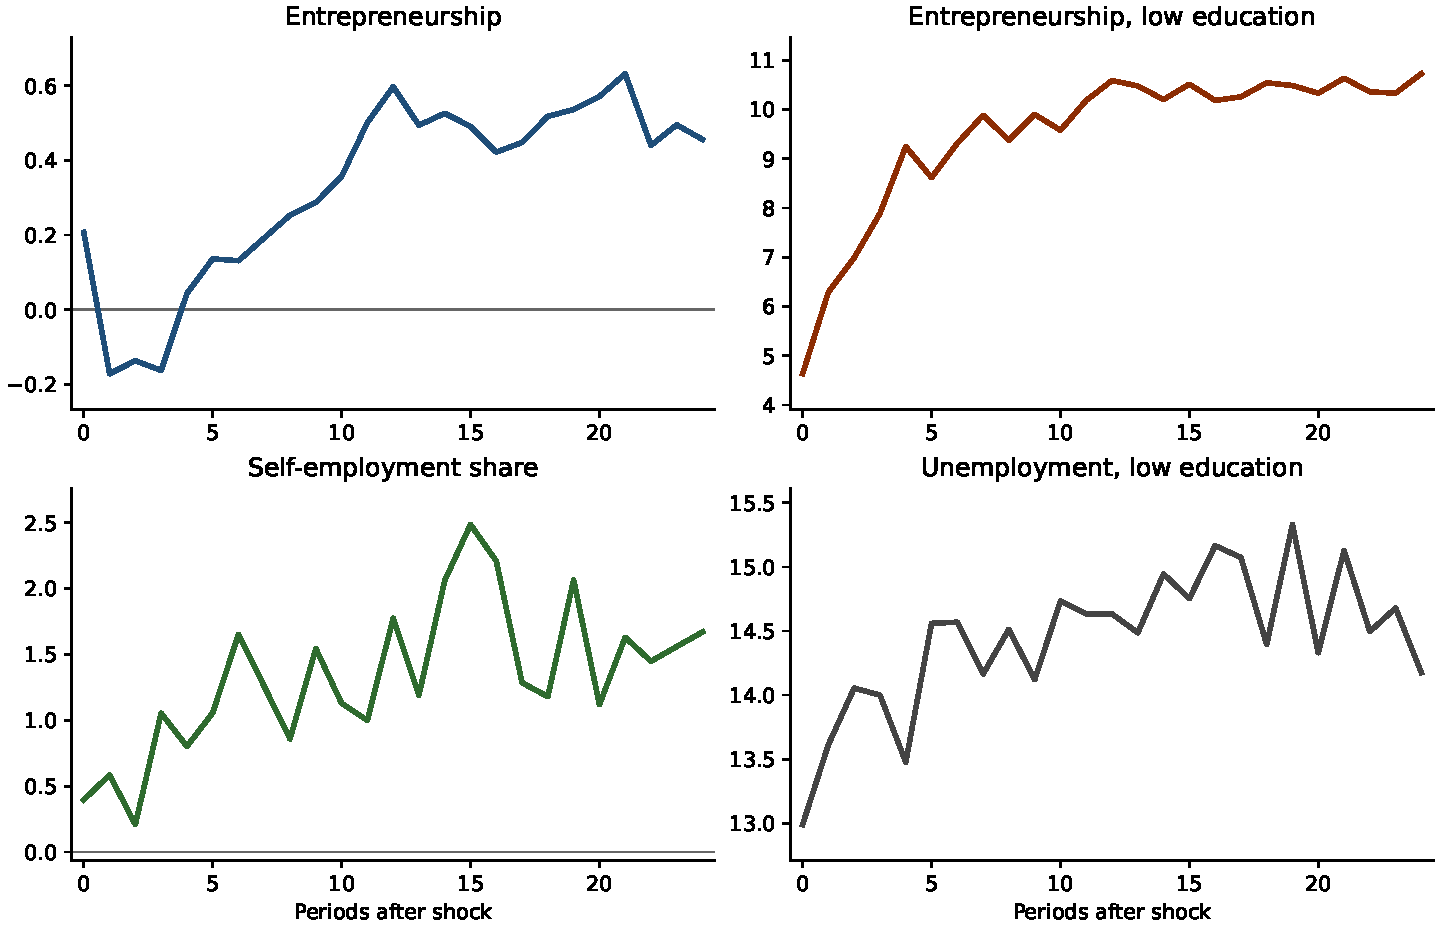
\includegraphics[width=0.95\textwidth]{../figures/case147_mit_lowedu_sep010_irf.pdf}\caption{MIT-style impulse responses for the low-education separation shock in the benchmark self-employment economy. Each panel reports percentage-point deviations from the benchmark transition start state.}\label{fig:case147_mit_lowedu_sep010_irf}\end{figure}

Figure \ref{fig:case147_mit_lowedu_sep010_irf} shows the transition
dynamics behind this steady-state comparison. Following the shock,
low-education unemployment rises on impact, and the entrepreneur pool
shifts modestly toward self-employment. The figure sharpens the same
interpretation as the steady-state comparison: a recession first worsens
labor-market outcomes for exposed individuals and then pushes some
marginal individuals into smaller-scale entrepreneurial activity.
This is the necessity-entry channel emphasized in the paper.

\FloatBarrier

\section{Conclusion}

This paper develops a quantitative framework for studying necessity
entrepreneurship as an equilibrium outcome of occupational choice
under labor-market frictions. By defining necessity and opportunity
entrepreneurship structurally, rather than through stated motives
or prior labor-market status, the paper provides a framework for analyzing
how outside options shape entrepreneurial entry.

The paper's central message is that entrepreneurship is a compositional
object, not just a scalar one. Labor-market conditions and policy
affect not only the level of entrepreneurial entry, but also whether
that entry takes the form of lower-scale self-employment or employer-oriented
entrepreneurship. This distinction matters for aggregate outcomes,
because the same rise in business ownership can reflect either productive
entrepreneurial opportunity or weak outside options.

The broader implication is that entrepreneurship should not be evaluated
by aggregate entry alone. Understanding who becomes an entrepreneur,
under what labor-market conditions, and at what scale is essential
for interpreting both entrepreneurial dynamics and the effects of policy.

\section*{\newpage}

\section*{Appendix}

\section*{Robustness}

The employer-threshold benchmark is disciplined locally around $f_{hire}=0.25$
rather than being treated as a single lucky parameter choice. The
appendix reports nearby values to show that the main composition result
is robust within a tight bracket.

\begin{table}[H]
\caption{Employer-threshold cost robustness in the benchmark baseline equilibrium}
\label{tab:self_employment_fhire_robustness_baseline}
\centering
\small
\begin{tabular}{|l|c|c|c|}
\hline
 & $f_{\mathrm{hire}}=0.15$ & $f_{\mathrm{hire}}=0.25$ & $f_{\mathrm{hire}}=0.35$ \\
\hline
Entrepreneur share (all households) & 0.1786 & 0.1781 & 0.1767 \\
\hline
Avg entrepreneur labor demand $n$ & 6.1274 & 6.1587 & 6.2336 \\
\hline
Avg entrepreneur capital $k$ & 97.8587 & 98.1596 & 98.8487 \\
\hline
\multicolumn{4}{|l|}{Self-employed among entrepreneurs ($n_h = 0$)} \\
\hline
All education & 0.5679 & 0.5768 & 0.5926 \\
\hline
Low education & 0.8190 & 0.8265 & 0.8494 \\
\hline
Middle education & 0.4482 & 0.4577 & 0.4637 \\
\hline
High education & 0.1109 & 0.1157 & 0.1215 \\
\hline
\multicolumn{4}{|l|}{Employer entrepreneurs among entrepreneurs ($n_h > 0$)} \\
\hline
All education & 0.4321 & 0.4232 & 0.4074 \\
\hline
Low education & 0.1810 & 0.1735 & 0.1506 \\
\hline
Middle education & 0.5518 & 0.5423 & 0.5363 \\
\hline
High education & 0.8891 & 0.8843 & 0.8785 \\
\hline
\end{tabular}
\end{table}

\begin{table}[H]
\caption{Employer-threshold cost robustness in the benchmark no-UI equilibrium}
\label{tab:self_employment_fhire_robustness_noui}
\centering
\small
\begin{tabular}{|l|c|c|c|}
\hline
 & $f_{\mathrm{hire}}=0.15$ & $f_{\mathrm{hire}}=0.25$ & $f_{\mathrm{hire}}=0.35$ \\
\hline
Entrepreneur share (all households) & 0.3348 & 0.3425 & 0.3401 \\
\hline
Avg entrepreneur labor demand $n$ & 2.6566 & 2.5529 & 2.6138 \\
\hline
Avg entrepreneur capital $k$ & 55.6364 & 54.0490 & 54.7019 \\
\hline
\multicolumn{4}{|l|}{Self-employed among entrepreneurs ($n_h = 0$)} \\
\hline
All education & 0.7321 & 0.7670 & 0.7710 \\
\hline
Low education & 0.8523 & 0.8711 & 0.8767 \\
\hline
Middle education & 0.7324 & 0.7732 & 0.7767 \\
\hline
High education & 0.4062 & 0.4408 & 0.4433 \\
\hline
\multicolumn{4}{|l|}{Employer entrepreneurs among entrepreneurs ($n_h > 0$)} \\
\hline
All education & 0.2679 & 0.2330 & 0.2290 \\
\hline
Low education & 0.1477 & 0.1289 & 0.1233 \\
\hline
Middle education & 0.2676 & 0.2268 & 0.2233 \\
\hline
High education & 0.5938 & 0.5592 & 0.5567 \\
\hline
\end{tabular}
\end{table}


Varying $f_{hire}$ between 0.15 and 0.35 barely changes the overall
entrepreneur share in the baseline economy, but it moves composition
in the expected direction: a higher employer threshold raises the
self-employed share and lowers the employer share. The same qualitative
pattern holds in the no-UI economy, where entrepreneurship remains
high and increasingly concentrated in self-employment.

The matched fixed-tax UI ladder delivers the same qualitative comparative
statics as the endogenous-tax benchmark. Lower UI still raises entrepreneurship
and shifts the entrepreneur pool toward smaller-scale self-employment
when the financing rule is held fixed. The benchmark results therefore
do not hinge on the fiscal closure used to finance unemployment insurance.

\section*{Measurement note}

To compare aggregate production across steady states, let $Y_{s}$ denote
simulated total output in steady state $s$ and let $H$ denote the
fixed number of simulated households. The aggregate output index reported
in the quantitative tables is
\[
\frac{Y_{s}/H}{Y_{0}/H}=\frac{Y_{s}}{Y_{0}},
\]
where $0$ denotes the benchmark steady state. So a value above one
means output per household, and therefore total output, is higher than
in the benchmark. Cutoff figures are omitted from the manuscript
appendix for brevity.

\section*{Computation}

Given the values for parameters, the discretized spaces $\Omega_{a}$
for $a$, $\Omega_{z}$ for $z$ and $\Omega_{x}$ for $x$. Each
agent draw a human capital level $h$ (interpreted as educational
attainment) at the beginning of the economy, which will be fixed henceforth.
$h$ will determine their labor productivity $z\in\Omega_{z}$, the
separation rate $\rho$, and managerial ability $x\in\Omega_{x}$.
Let $i_{w}=0$ indicating being entrepreneur, $i_{w}=1$ being employed
and $i_{w}=2$ being unemployed. The numerical algorithm works as
follows. 
\begin{enumerate}
\item Set a tolerance $\epsilon>0$. 
\item Guess $\Phi^{0}=\left(r^{0},w^{0},\rho^{0},\tau^{0}_{y}\right)$.
Solve for optimal household behavior: 
\[
f:\left(\varphi;\Phi\right)\rightarrow\left(c,a',\mathcal{I}_{e},n,k\right),
\]
where $\varphi=\left\{ h,z,x,a,i_{w}\right\} $. We will use the method
of value function iteration as follows.
\begin{enumerate}
\item Guess value function $\mathbf{V}{}^{0}\left(\varphi;\Phi^{0}\right)$
and policy functions $f^{0}\left(\varphi;\Phi^{0}\right)$. 
\item Calculate the cutoff values of $x^{*}_{u}$ (for previously unemployed
worker, or entrepreneur) and $x^{*}_{n}$ (for previously employed
worker) via the following conditions. 
\begin{align}
\widetilde{w}_{u}= & \pi(x^{*}_{u})=\max_{k,n_{h}\geq0}\left\{ x^{*}_{u}k^{\alpha}\left(\ell_{e}+\xi zn_{h}\right)^{\gamma}-w(1+\psi\tau)zn_{h}-rk-\frac{\kappa\rho zn_{h}}{q(\theta)}-f_{hire}\mathbf{1}\{n_{h}>0\}\right\} \label{eq:xstar_u}\\
\widetilde{w}_{n}= & \pi(x^{*}_{n})=\max_{k,n_{h}\geq0}\left\{ x^{*}_{n}k^{\alpha}\left(\ell_{e}+\xi zn_{h}\right)^{\gamma}-w(1+\psi\tau)zn_{h}-rk-\frac{\kappa\rho zn_{h}}{q(\theta)}-f_{hire}\mathbf{1}\{n_{h}>0\}\right\} \label{eq:xstar_n}
\end{align}
where $\widetilde{w}_{n}$ and $\widetilde{w}_{u}$ denote the expected
compensation for the employed worker and unemployed worker respectively.
More specifically, 
\begin{align}
\widetilde{w}_{n} & =(1-\rho)\left\{ zw(1-(1-\psi)\tau)\right\} +\rho b\label{eq:income_n}\\
\widetilde{w}_{u} & =p(\theta)\left\{ zw(1-(1-\psi)\tau)\right\} p(\theta))b.\label{eq:income_u}
\end{align}
Noting that the separation rate $\rho$ is pre-determined by the individual's
initial human capital level $h$. 
\item Update value and policy functions: 
\begin{align}
\mathbf{V}^{1}(h,z,x,a,i_{w})=\label{eq:V_overall}\\
\max_{\left\{ a',c,\mathcal{I}_{e}\right\} }\left\{ \begin{array}{c}
\iota_{i_{w}=0}\cdot\left[\begin{array}{c}
(1-\mathcal{I}_{e})\cdot\mathbb{E}_{p(\theta)}\left(V_{w}+\beta\mathbb{E}\mathbf{V}^{0}(h,z',x',a',i'_{w})\right)\\
+\mathcal{I}_{e}\cdot\left(V_{e}+\beta\mathbb{E}\mathbf{V}^{0}(h,z',x',a',i'_{w}=2)\right)
\end{array}\right]+\\
\iota_{i_{w}=1}\cdot\left[\begin{array}{c}
(1-\mathcal{I}_{e})\cdot\mathbb{E}_{\rho}\left(V_{w}+\beta\mathbb{E}\mathbf{V}^{0}(h,z',x',a',i'_{w})\right)\\
+\mathcal{I}_{e}\cdot\left(V_{e}+\beta\mathbb{E}\mathbf{V}^{0}(h,z',x',a',i'_{w}=2)\right)
\end{array}\right]+\\
\iota_{i_{w}=2}\cdot\left[\begin{array}{c}
(1-\mathcal{I}_{e})\cdot\mathbb{E}_{p(\theta)}\left(V_{w}+\beta\mathbb{E}\mathbf{V}^{0}(h,z',x',a',i'_{w})\right)\\
+\mathcal{I}_{e}\cdot\left(V_{e}+\beta\mathbb{E}\mathbf{V}^{0}(h,z',x',a',i'_{w}=2)\right)
\end{array}\right]
\end{array}\right\} \nonumber \\
f^{1}\left(\varphi;\Phi^{0}\right)=\arg\max\mathbf{V}^{1}\left(\varphi;\Phi^{0}\right)\nonumber 
\end{align}
where $\mathbb{E}_{p(\theta)}\left(V_{w}+\beta\mathbb{E}\mathbf{V}(a',x',i'_{w})\right)$
denotes the expected payoff for the individual who is previously unemployed
worker, or entrepreneur, and decides to look for paid job, while $\mathbb{E}_{\rho}\left(V_{w}+\beta\mathbb{E}\mathbf{V}(a',x',i'_{w})\right)$
represents the expected payoff for the previously employed worker
who decide to stay in workplace. 
\begin{align}
\mathbb{E}_{p(\theta)}\left(V_{w}+\beta\mathbb{E}\mathbf{V}(h,z',x',a',i'_{w})\right) & =p(\theta)\left(V_{n}+\beta\mathbb{E}\mathbf{V}(h,z',x',a',i'_{w}=1)\right)\label{eq:V_u}\\
 & +(1-p(\theta))\left(V_{u}+\beta\mathbb{E}\mathbf{V}(h,z',x',a',i'_{w}=0)\right)\nonumber \\
\mathbb{E}_{\rho}\left(V_{w}+\beta\mathbb{E}\mathbf{V}(h,z',x',a',i'_{w})\right) & =(1-\rho)\left(V_{n}+\beta\mathbb{E}\mathbf{V}(h,z',x',a',i'_{w}=1)\right)\label{eq:V_w}\\
 & +\rho\left(V_{u}+\beta\mathbb{E}\mathbf{V}(h,z',x',a',i'_{w}=0)\right)\nonumber 
\end{align}
To simplify the analysis, we assume that the individual who was previously
employed and newly separated from the firm is not allowed to search
for job at the current period. The measure for the individuals who
are looking for jobs, $u_{t}$, the total vacancies $v_{t}$, and
job matching rate $\theta_{n,t}$ are given as follows. 
\begin{align}
u_{t} & =\left(\int_{x}\iota_{i_{w}=0}+\int_{x}\iota_{i_{w}=2}\right)\cdot\int^{x^{*}_{u}}_{0}\label{eq:measure_u}\\
v_{t} & =\int_{x}\iota_{i_{w}=1}\cdot\rho\label{eq:measure_v}\\
\theta_{n,t} & =\bar{m}\left(\frac{v_{t}}{u_{t}}\right)^{1-\mu}\label{eq:measure_matching}
\end{align}
Note that we can write the above value functions explicitly as a system
of sub-problems: $P^{i_{w}=0}_{x<x^{*}_{u}}$ , $P^{i_{w}=0}_{x\geq x^{*}_{u}}$,
$P^{i_{w}=1}_{x<x^{*}_{n}}$ , $P^{i_{w}=1}_{x\geq x^{*}_{n}}$, $P^{i_{w}=2}_{x<x^{*}_{u}}$
, $P^{i_{w}=2}_{x\geq x^{*}_{u}}$, which correspond to the dynamic
programing problem for i). previously self-employed with $x<x^{*}_{u}$;
ii). previously self-employed with $x\geq x^{*}_{u}$; iii). previously
employed with $x<x^{*}_{n}$; iv). previously employed with $x\geq x^{*}_{n}$;
v). previously unemployed with $x<x^{*}_{u}$; vi). previously unemployed
with $h\geq h^{*}_{u}$. To economize the space, we only provide the
details for $P^{i_{w}=0}_{x<x^{*}_{u}}$ , and $P^{i_{w}=0}_{x\geq x^{*}_{u}}$
as follows. \\
 $\left(P^{i_{w}=0}_{x<x^{*}_{u}}\right)$: 
\begin{equation}
\mathbf{V}^{1}(h,z,x<x^{*}_{u},a,i_{w}=0)=\max_{a'_{n},a'_{u}}\left\{ \begin{array}{c}
p(\theta)\left(u(c_{n})+\beta\mathbb{E}\mathbf{V}^{0}(h,z',x',a'_{n},i'_{w}=1)\right)\\
+(1-p(\theta))\left(u(c_{u})+\beta\mathbb{E}\mathbf{V}^{0}(h,z',x',a'_{u},i'_{w}=0)\right)
\end{array}\right\} \label{eq:V_iw0_xl}
\end{equation}
s.t. 
\begin{align}
c_{n}+a'_{n} & \leq(1-\tilde{r}-\delta)a+zw(1-(1-\psi)\tau),\text{if matched with a firm}\label{eq:bdg_iw0_xl_1}\\
c_{u}+a'_{u} & \leq(1-\tilde{r}-\delta)a+b,\text{if unemployed}\label{eq:bdg_iw0_xl_2}
\end{align}
$\left(P^{i_{w}=0}_{x\geq x^{*}_{u}}\right)$: 
\begin{equation}
\mathbf{V}^{1}(h,z,x\geq x^{*}_{u},a,i_{w}=0)=\max_{a_{e}',k,n_{h}\geq0}\left\{ u(c_{e})+\chi_{se}\mathbf{1}\{n_{h}=0\}+\chi_{emp}\mathbf{1}\{n_{h}>0\}+\beta\left[(1-\rho_{e}(h))\mathbb{E}\mathbf{V}^{0}(h,z',x',a_{e}',i'_{w}=2)+\rho_{e}(h)\mathbb{E}\mathbf{V}^{0}_{0}(h,z',x',a_{e}',i'_{w}=0)\right]\right\} \label{eq:V_iw0_xh}
\end{equation}
s.t. 
\begin{equation}
c_{e}+a_{e}'\leq(1-\tilde{r}-\delta)a+\pi(k,n_{h},x;\tilde{r},w,\tau)\label{eq:bdg_iw0_xh}
\end{equation}
where 
\begin{equation}
\pi(k,n_{h},x;\tilde{r},w,\tau)=xk^{\alpha}\left(\ell_{e}+\xi zn_{h}\right)^{\gamma}-w(1+\psi\tau)zn_{h}-rk-\frac{\kappa\rho zn_{h}}{q(\theta)}-f_{hire}\mathbf{1}\{n_{h}>0\}.\label{eq:profit_emtrepreneur}
\end{equation}
\item Stop if $\max\left\{ \left|\mathbf{V}^{1}-\mathbf{V}^{0}\right|,\left|f^{1}-f^{0}\right|\right\} \leq\epsilon$.
Set $\mathbf{V}^{*}=\mathbf{V}^{1}$, and $f^{*}=f^{1}$. Otherwise,
set $\mathbf{V}^{0}=\mathbf{V}^{1}$, $f^{0}=f^{1}$ and repeat from
step (c). 
\end{enumerate}
\item Generate a large number of individuals, $N=100000$. For each agent
$j$ assign a vector of initial condition $\left(h^{j}_{t},z^{j}_{0},x^{j}_{0},a^{j}_{0},i^{j}_{w,0}\right)$,
where $x^{j}_{0}\sim\Omega_{x}$, $z^{j}_{0}\in\Omega_{z}$, $i^{j}_{w,0}\in\Omega_{w}$. 
\item Simulate the economy for $T$ periods, where $T$ is sufficiently
large. 
\item Calculate the following statistics from the simulated path $\left\{ h^{j}_{t},z^{j}_{t},x^{j}_{t},a^{j}_{t},i^{j}_{w,t},\mathcal{I}^{j}_{e,t},n^{j}_{t},k^{j}_{t}\right\} ^{T}_{t=0}$.
\begin{align}
LS^{0} & =\frac{\sum^{N}_{j=1}\left(\iota_{i_{w}=1}\cdot z^{j}\right)}{N}\label{eq:agg_simulation_1}\\
KS^{0} & =\frac{\sum^{N}_{j=1}\left(\iota_{i_{w}=0}\cdot a^{j}+\iota_{i_{w}=1}\cdot a^{j}+\iota_{i_{w}=2}\cdot a^{j}-\iota_{i_{w}=0}\cdot k^{j}\right)}{\sum^{N}_{j=1}a^{j}}\label{eq:agg_simulation_2}\\
u_{t} & =\left(\int_{h}\iota_{i_{w}=0}+\int_{h}\iota_{i_{w}=2}\right)\cdot\int^{h^{*}_{u}}_{0}\\
v_{t} & =\int_{h}\iota_{i_{w}=1}\cdot\rho\\
p(\theta)_{t} & =\bar{m}\left(\frac{v_{t}}{u_{t}}\right)^{1-\mu}\\
G & =\int\tau wz
\end{align}
and $\tau^{1}_{y}$ that balances the government's budget. 
\item Stop and set $\left(r^{*},w^{*},\theta^{*}\right)=\left(r^{0},w^{0},\theta^{0}\right)$,
if $\max\left\{ LS^{0},KS^{0},\left|\theta^{1}_{n}-\theta^{0}_{n}\right|\right\} \leq\epsilon$.
Otherwise, update aggregate variables (restart from step 2): 
\begin{align*}
r^{0} & =\chi r^{0}+(1-\chi)r^{1}\left(KS^{0}\right)\\
w^{0} & =\chi w^{0}+(1-\chi)w^{1}\left(LS^{0}\right)\\
p(\theta)^{0} & =\chi p(\theta)^{0}+(1-\chi)p(\theta)^{1}\\
\tau^{0}_{y} & =\chi\tau^{0}_{y}+(1-\chi)\tau^{1}_{y}
\end{align*}
where $\chi\in(0,1)$ is the step for updating aggregate variables. 
\end{enumerate}

\section*{}

\section*{Appendix Search and Matching}

I am not sure how much of this is needed for coding purposes but this
is the standard search and matching model. The stock of employed workers
$n_{t}$ can be expressed as the current pool of workers who did not
separate from firms, plus new hires

\[
n_{t}=(1-\rho)n_{t-1}+m_{t-1}
\]
The matching function is Cobb-Douglass where

\[
m_{t}=\bar{m}v^{1-\mu}_{t}u^{\mu}_{t}
\]
$\bar{m}$ is a match efficiency parameter , $v$ is vacancies, $u$
is unemployment, and match elasticity is $0<\mu<1$.The hiring rate
can be defined for firms as total number of new hires to the number
of vacancies

\[
q(\theta_{t})=\frac{m_{t}}{v_{t}}=\bar{m}\theta^{-\mu}_{t}
\]
where $\theta_{t}=\frac{v_{t}}{u_{t}}$is aggregate labour market
tightness. Similarly we can define this from the perspective of the
worker in the job-finding rate.

\[
p(\theta_{t})=\frac{m_{t}}{u_{t}}=\bar{m}\theta^{1-\mu}_{t}
\]
The Job Creation Condition determines the amount of new vacancies
an employer will post. In our model, most workers are on rolling contracts,
so firms only need to post new vacancies after some workers separate
from these rolling contracts. Usually in search and matching models
the wage is determined ex-post of matching by Nash bargaining between
the employer and employee. However, in our span-of-control model the
wage has already been determined ex ante, as the wage is an endogenous
variable that determines occupational choice. The marginal benefit
that the new employee would bring to the firm is expressed as $A$
(which can be derived from the firms production function, $\gamma Xk^{\alpha}(zn)^{\gamma-1}$).
The $JCC\text{ can be then expressed as the costs of replacing out workers on the \ensuremath{LHS} and the expected benefit on the \ensuremath{RHS.}}$

\[
\frac{\kappa}{q(\theta_{t})}=A-w_{t}+\beta E_{t}\left[A-w_{t+1}+(1-\rho)\frac{\kappa}{q(\theta_{t+1})}\right]
\]
where $\kappa$ is the cost of posting a vacancy. %
\begin{comment}
This is different from the standard JCC as usually production starts
the period after matching so the JCC would be $\frac{\kappa}{q(\theta_{t})}=+\beta E_{t}\left[A-w_{t+1}+(1-\rho)\frac{\kappa}{q(\theta_{t+1})}\right].$
See alternative timing version to think about the problem this way,
I am not sure it makes much difference. 
\end{comment}


\subsection*{Matching Steady States}

To find the steady state of the employment equation $n_{t}=(1-\rho)n_{t-1}+m_{t-1}$,
we use the fact that $u=(1-n)$ and $m_{t}=\bar{m}v^{1-\mu}_{t}u^{\mu}_{t}.$
Substituting and getting rid of time subscript gives $(1-u)=(1-\rho)(1-u)+\bar{m}v^{1-\mu}u^{\mu}$
which simplifies to $\bar{m}v^{1-\mu}_{t}u^{\mu}_{t}=$$\rho(1-u)$.
Making $v\text{\,the subject of the foruma gives us the Beveridge curve.}$

\[
v=\left(\frac{\rho(1-u)}{\bar{mu}}\right)^{1-\mu}u
\]
The steady state for the JCC can be found by using $\frac{\kappa}{q(\theta_{t})}=A-w_{t}+\beta E_{t}\left[A-w_{t+1}+(1-\rho)\frac{\kappa}{q(\theta_{t+1})}\right]$
and $q(\theta_{t})=\bar{m}\theta^{-\mu}_{t}=\bar{m}\left(\frac{v_{t}}{u_{t}}\right)^{-\mu}$.
Substituting and getting rid of time subscripts yields 
\[
\frac{\kappa}{\bar{m}}\left(\frac{v}{u}\right)^{\mu}=A-w_{t}+\beta\left[A-w+(1-\rho)\frac{\kappa}{\bar{m}}\left(\frac{v}{u}\right)^{\mu}\right]
\]

Simplifying yields the steady state of the JCC

\[
1-\beta(1-\rho)\frac{\kappa}{\bar{m}}\left(\frac{v}{u}\right)^{\mu}=(1+\beta)\left[A-w\right]
\]

 \bibliographystyle{apalike}
\bibliography{../../../_shared/references/global_references}

\end{document}
